\section{Regresión lineal simple y correlación}
Cuando trabajamos con dos variables cuantitativas a la vez (datos bivariados), el objetivo
cambia: ya no miramos un solo grupo, sino que buscamos saber si una variable se relaciona con
la otra, en qué sentido y con qué intensidad. Para esto usamos dos herramientas esenciales:
\begin{itemize}
  \item \textbf{El coeficiente de correlación de Pearson ($r$):} mide la fuerza de la relación    entre $-1$ y $+1$.
  \item \textbf{La regresión lineal (mínimos cuadrados):} encuentra la ecuación de la recta
    $\hat{y} = b_0 + b_1 x$ que mejor se ajusta a los puntos para hacer predicciones precisas.
\end{itemize}

\AnalisisDescriptivo
Para evaluar el impacto de las horas de estudio semanal ($x$) sobre el puntaje matemático
($y$), analizamos una muestra de $n = 30$ alumnos. Sus estadísticos descriptivos son:

\begin{TablaDatosFlexible}{L{0.34\linewidth} C{0.24\linewidth} C{0.24\linewidth}}{\textbf{Métrica} & \textbf{Horas de estudio ($x$)} & \textbf{Puntaje matemático ($y$)}}

\TablaFilaFlexible{Cantidad de datos ($n$) & 30 & 30}
\TablaFilaFlexible{Sumatoria & 206 & 2519}
\TablaFilaFlexible{Promedio (media) & 6,87 & 83,97}
\TablaFilaFlexible{Varianza ($S^2$) & 2,12 & 17,34}
\TablaFilaFlexible{Desviación estándar ($S$) & 1,46 & 4,16}
\TablaFilaFlexible{Coef. de variación (CV) & 21,20\% & 4,96\%}

\end{TablaDatosFlexible}

\subsection{Cálculos intermedios}
Antes de armar la recta necesitamos las sumas de cuadrados y el producto cruzado de las dos
variables. Con los valores de la tabla anterior ($\sum x = 206$, $\sum y = 2519$,
$\sum x^2 = 1476$, $\sum y^2 = 212015$ y $\sum xy = 17368$):
\begin{equation*}
  SC_x = \sum x^2 - \frac{(\sum x)^2}{n} = 1476 - \frac{206^2}{30}
       = 1476 - 1414{,}53 = 61{,}47
\end{equation*}
\begin{equation*}
  SC_y = \sum y^2 - \frac{(\sum y)^2}{n} = 212015 - \frac{2519^2}{30}
       = 212015 - 211512{,}03 = 502{,}97
\end{equation*}
\begin{equation*}
  S_{xy} = \sum xy - \frac{(\sum x)(\sum y)}{n} = 17368 - \frac{206 \cdot 2519}{30}
         = 17368 - 17297{,}13 = 70{,}87
\end{equation*}

% --------------------------------------------------------------------------------------------------

\subsection{La recta de regresión}
\subsubsection{Pendiente ($b_1$)}
\begin{equation*}
  b_1 = \frac{S_{xy}}{SC_x} = \frac{70{,}87}{61{,}47} = \mathbf{1{,}153}
\end{equation*}
\PalabraClave{Interpretación:} Por cada hora extra de estudio semanal, el puntaje estimado en
matemáticas aumenta en 1,153 puntos.

\subsubsection{Ordenada al origen ($b_0$)}
\begin{equation*}
  b_0 = \bar{y} - b_1 \cdot \bar{x} = 83{,}97 - (1{,}153 \cdot 6{,}87)
      = 83{,}97 - 7{,}92 = \mathbf{76{,}05}
\end{equation*}
\PalabraClave{Interpretación:} Si un alumno estudia 0 horas, su puntaje base estimado es de
76,05 puntos.

La ecuación completa de la recta de mínimos cuadrados queda entonces:
\begin{equation*}
  \hat{y} = 76{,}05 + 1{,}153x
\end{equation*}

% --------------------------------------------------------------------------------------------------

\subsection{Coeficiente de correlación ($r$)}
\begin{equation*}
  r = \frac{S_{xy}}{\sqrt{SC_x \cdot SC_y}} = \frac{70{,}87}{\sqrt{61{,}47 \cdot 502{,}97}}
    = \frac{70{,}87}{175{,}83} = \mathbf{0{,}403}
\end{equation*}
\PalabraClave{Interpretación:} Existe una asociación lineal positiva y de intensidad moderada
entre las horas de estudio semanales y el puntaje obtenido por los 30 alumnos.

\TituloGrafico{Recta de ajuste de mínimos cuadrados}
\begin{figure}[H]
    \centering
    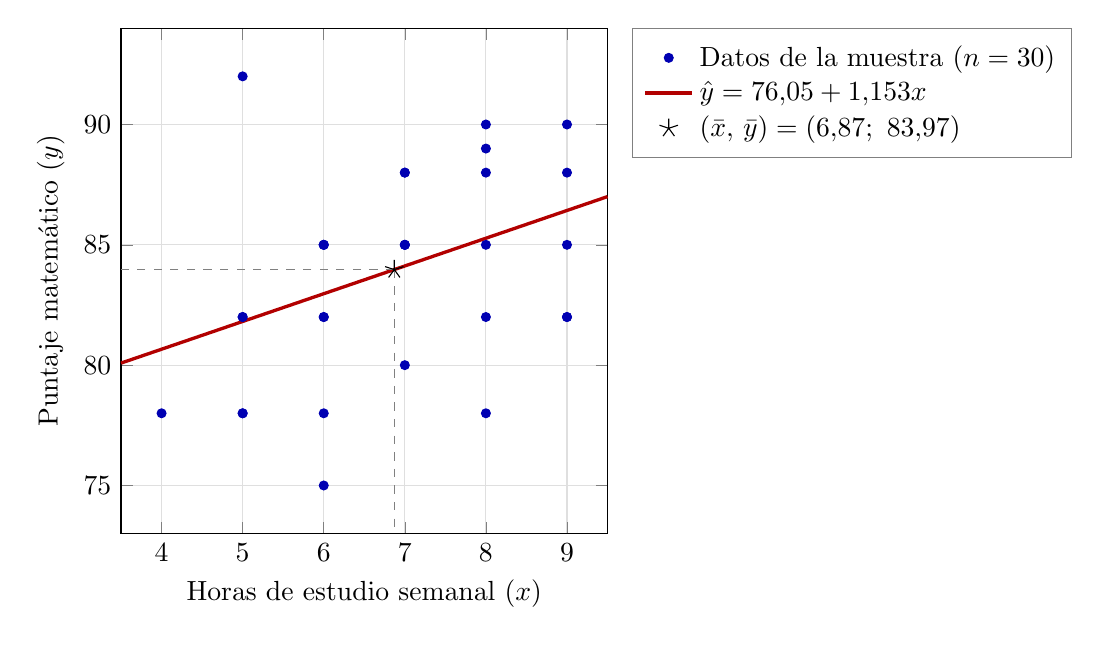
\begin{tikzpicture}
        \begin{axis}[
            width=0.64\textwidth,
            height=8cm,
            xlabel={Horas de estudio semanal ($x$)},
            ylabel={Puntaje matemático ($y$)},
            xmin=3.5, xmax=9.5,
            ymin=73, ymax=94,
            xtick={4,5,6,7,8,9},
            ytick={75,80,85,90},
            grid=major,
            grid style={gray!25},
            legend style={at={(1.05,1.0)}, anchor=north west, fill=white, draw=black!50,
                fill opacity=1, text opacity=1, inner sep=4pt, cells={anchor=west}},
            legend cell align=left,
            clip=false,
        ]
            % Dispersión: los 30 pares (horas, puntaje) de la muestra.
            \addplot[only marks, mark=*, mark size=1.6pt, blue!70!black] coordinates {
                (6,85) (8,78) (5,92) (7,80) (6,75) (9,88) (5,82) (6,85) (4,78) (8,89)
                (7,85) (9,90) (6,82) (5,78) (8,85) (7,88) (6,82) (9,85) (8,90) (5,82)
                (6,78) (7,85) (8,88) (9,82) (6,85) (7,88) (8,82) (5,78) (7,85) (9,82)
            };
            \addlegendentry{Datos de la muestra ($n = 30$)}
            % Recta de regresión: y = 76,05 + 1,153x.
            \addplot[red!70!black, very thick, domain=3.5:9.5] {76.05 + 1.153*x};
            \addlegendentry{$\hat{y} = 76{,}05 + 1{,}153x$}
            % Punto centróide: la recta pasa por (x̄, ȳ).
            \addplot[only marks, mark=star, mark size=3.5pt, black] coordinates {(6.87,83.97)};
            \addlegendentry{$(\bar{x},\, \bar{y}) = (6{,}87;\ 83{,}97)$}
            % Líneas guía hacia los ejes.
            \draw[gray, dashed, thin] (axis cs:6.87,83.97) -- (axis cs:6.87,73);
            \draw[gray, dashed, thin] (axis cs:6.87,83.97) -- (axis cs:3.5,83.97);
        \end{axis}
    \end{tikzpicture}
    \caption{Dispersión de los 30 alumnos de la muestra (puntos azules) con la recta de
    regresión $\hat{y} = 76{,}05 + 1{,}153x$ (línea roja). La estrella negra marca el promedio
    de la muestra $(6{,}87;\ 83{,}97)$, punto por el que la recta siempre pasa.}
    \label{fig:regresion_recta}
\end{figure}

\Interpretacion
La recta $\hat{y} = 76{,}05 + 1{,}153x$ resume la relación entre ambas variables: cada hora
semanal adicional de estudio se asocia con un aumento esperado de 1,153 puntos en el puntaje de
matemáticas. El coeficiente de correlación $r = 0{,}403$ confirma una asociación positiva de
intensidad moderada: el tiempo de estudio explica en parte el rendimiento, pero no es el único
factor. Como el modelo es una estimación, las predicciones deben interpretarse como valores
esperados del grupo y no como notas garantizadas para cada alumno.